%!TEX TS-program = xelatex
%!TEX encoding = UTF-8 Unicode


\documentclass[12pt]{extarticle}
% extarticle is like article but can handle 8pt, 9pt, 10pt, 11pt, 12pt, 14pt, 17pt, and 20pt text

\def \ititle {Philosophical Psychology}

\def \isubtitle {Lecture 11}

\def \iauthor {Stephen A. Butterfill}
\def \iemail{s.butterfill@warwick.ac.uk}
\date{}

%for strikethrough
\usepackage[normalem]{ulem}

\input{$HOME/latex_imports/preamble_steve_handout}

%\bibpunct{}{}{,}{s}{}{,}  %use superscript TICS style bib
%remove hanging indent for TICS style bib
%TODO doesnt work
\setlength{\bibhang}{0em}
%\setlength{\bibsep}{0.5em}


%itemize bullet should be dash
\renewcommand{\labelitemi}{$-$}

\begin{document}

\begin{multicols*}{3}

\setlength\footnotesep{1em}


\bibliographystyle{newapa} %apalike

%\maketitle
%\tableofcontents




%---------------
%--- start paste



\def \ititle {11: The Motor Theory of Goal Tracking}

\begin{center}

{\Large

\textbf{\ititle}

}



\iemail %

\end{center}

 

 
\section{Pure Goal Tracking}
 
An account of \emph{pure goal tracking} is an account of how you could 
in principle infer facts about the goals to which actions are directed from
facts about joint displacements, bodily configurations and their effects 
(e.g. sounds).

Goal tracking matters for (i) identifying intentions and other mental states (\citealp[p.~861]{Newtson:1977dw}; \citealp[p.~708]{Baldwin:2001rn}); (ii)  efficiently representing events \citep{Kurby:2008bk}; (iii) identifying the likely effects of actions \citep{Byrne:1999jk}; (iv) predicting when an event likely to be of interest will occur \citep[p.~121]{Swallow:2008cf};
and (v) learning through observation how to do things \citep{Byrne:2003wx}.

\dots And of course a special case of pure behaviour reading, ‘speech perception’, underpins communication by language in humans.
 
\begin{center}
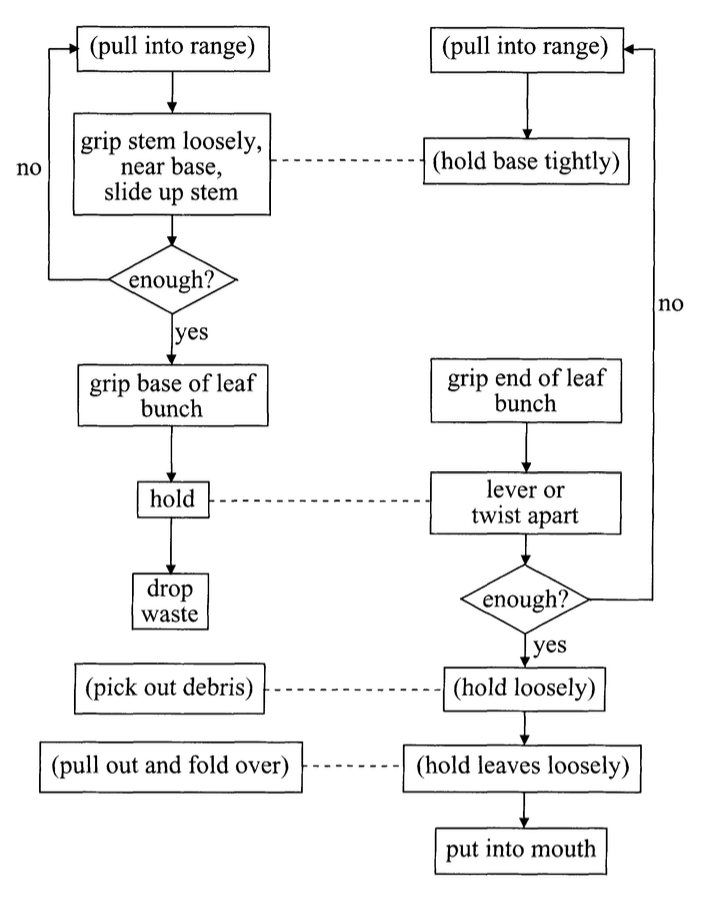
\includegraphics[scale=0.3]{img/byrne_2003_fig1.png}
\end{center}
‘great apes [are] able to acquire complex and elaborate local traditions of food
acquisition, some of them involving tool use’ \citep[p~513]{Byrne:2003wx}
 
 
 
\section{The Teleological Stance}
 
‘an action can be explained by a goal state if, and only if, it is seen as  the  most justifiable action towards that goal state that is available within the constraints of reality’
\citep[p.~255]{Csibra:1998cx}
 
\columnbreak

These facts:
%
\begin{enumerate}
%
\item action $a$ is directed to some goal;
%
\item actions of $a$'s type are normally capable of being means of realising outcomes of $G$'s type in situations with the salient (to any concerned) features of this situation;
% 
\item no alternative type of action is both 
typically available to agents of this type 
and also 
such that actions of this type would be normally be significantly better\footnotemark \ means of realising outcome $G$ in situations with the salient features of this situation;
%
\item the occurrence of outcome $G$ is typically desirable for agents of this type;
%
\end{enumerate}
%
and
%
\begin{enumerate}[resume]
\item there is no other outcome, $G'$, 
the occurrence of which would be at least comparably desirable for agents of this type 
and where (2) and (3) both hold of $G'$ and $a$
%
%where
%	the occurrence of $G'$ would be at least comparably desirable for agents of this type 
%%where
%%	$G$'s occurrence is not a means to $G'$'s nor conversely,
%and
%where  
%	(2) and (3) both hold of $G'$ and $a$
\end{enumerate}
%
may jointly constitute defeasible evidence for the conclusion that:
%
\begin{enumerate}[resume]
\item $G$ is a goal to which action $a$ is directed.
\end{enumerate}
%

  Claim: the above inference, from (1)-(5) to (6), is a route to knowledge of the goals of actions in this sense:
in some cases
it would be possible to know the premises without already knowing the conclusion;
and, 
in some of those cases,
knowing the premises could put one in a position to know the conclusion.

An action of type $a'$ is a \emph{better} means of realising outcome $G$ in a given situation than an action of type $a$ if, for instance, actions of type $a'$ normally involve less effort than actions of type $a$
in situations with the salient features of this situation
and everything else is equal;
or if, for example, actions of type $a'$ are normally more likely to realise outcome $G$ than actions of type $a$
in situations with the salient features of this situation
and everything else is equal.


 

 
\section{The Motor Theory of Goal Tracking}
 

\subsection{The Simple View}
‘when taking the teleological stance one-year-olds apply the same
inferential principle of rational action that drives everyday mentalistic
reasoning about intentional actions in adults’
(\citealp{Gergely:2003gb}; compare \citealp{Csibra:2003jv}, \citealp[p.~259]{Csibra:1998cx} )

‘Such calculations require detailed knowledge of biomechanical factors that 
determine the motion capabilities and energy expenditure of agents. However, 
in the absence of such knowledge, one can appeal to heuristics that approximate 
the results of these calculations on the basis of knowledge in other domains 
that is certainly available to young infants. For example, the length of 
pathways can be assessed by geometrical calculations, taking also into 
account some physical factors (like the impenetrability of solid objects). 
Similarly, the fewer steps an action sequence takes, the less effort it might 
require, and so infants’ numerical competence can also contribute to efficiency 
evaluation.’ \citep{csibra:2013_teleological}
 
\subsection{The Motor Theory}

According to the \emph{Motor Theory of Goal Tracking}, infants (and adults) sometimes track the
goals of others’ by means of motor processes \citep[see][for details]{sinigaglia:2015_puzzle}.
 
More carefully  the \emph{Motor Theory of Goal Tracking} states that: 
\begin{enumerate}
\item in action observation, possible outcomes of observed actions are represented motorically;
\item these representations trigger motor processes much as if the observer were performing actions directed to the outcomes;
\item such processes generates predictions;
\item a triggering representation is weakened if the predictions it generates fail.
\end{enumerate}
The result is that, often enough, the only only outcomes to which the observed action is a means
are represented strongly.
 
 
\begin{center}

  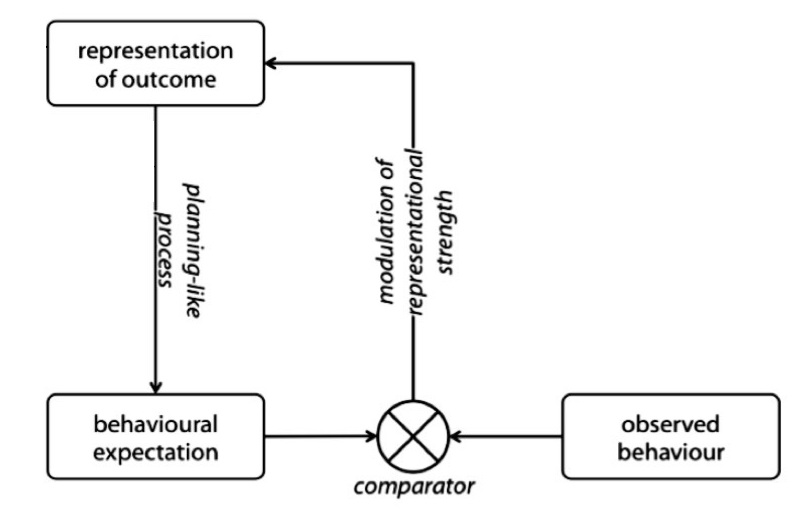
\includegraphics[scale=0.32]{fig/motor_theory.jpg}
  
  \end{center}

\section{Marr’s Threefold Distinction}
 
\citet[p.~22ff]{Marr:1982kx} distinguishes:
 
\begin{itemize}
 
\item computational description---What is the thing for and how does it achieve this?
 
\item representations and algorithms---How are the inputs and outputs represented, and how is the transformation accomplished?
 
\item hardware implementation---How are the representations and algorithms physically realised?
 
\end{itemize}



\vfill


%--- end paste
%---------------

\footnotesize
\bibliography{$HOME/endnote/phd_biblio}

\end{multicols*}

\end{document}
